\documentclass[a4paper, 12pt]{book}

\usepackage{amsthm}
\usepackage{geometry}
\usepackage{color}
% از این بسته برای محیط کدهای منبع، موجود در نوشته‌ها، استفاده می‌گردد.
\usepackage{listings}
\usepackage{hyperref}
\usepackage{graphicx}
\hypersetup{%
    pdfborder = {0 0 0}
}

\geometry{a4paper, tmargin=20mm, bmargin=20mm, lmargin=20mm, rmargin=20mm, footskip=10mm}
%%%%%%%%%%%%%%%%%%%%%%%%%%%%%%%%%%%%%%%%%%%%%%%%%%%%%%%%%%
\renewcommand{\sectionmark}[1]{%
\markright{\thesection\ #1}}
% بسته‌ای برای ظاهر شدن «مراجع» و «نمایه» در فهرست مطالب
\usepackage[nottoc]{tocbibind}
%
% دستوری برای تعریف واژه‌نامه انگلیسی به فارسی
%
\newcommand\persiangloss[2]{#1\dotfill \lr{#2}\\}
% دستوری برای تعریف واژه‌نامه فارسی به انگلیسی 
\newcommand\englishgloss[2]{#2\dotfill \lr{#1}\\}
%%%%%%%%%%%%%%%%%%%%%%%%%%%%%%%%%%%%%%%%%%%%%%%%%%%%
\usepackage{xepersian}
\settextfont[Scale=1.0]{XB Niloofar}
\setlatintextfont{Linux Libertine O}
\setdigitfont{XB Yas}

\definecolor{dkgreen}{rgb}{0,0.6,0}
\definecolor{gray}{rgb}{0.85,0.85,0.85}
\definecolor{mauve}{rgb}{0.58,0,0.82}
\definecolor{black}{rgb}{0,0,0}
\definecolor{red}{rgb}{1,0,0}

\lstset{
	language=bash,
	showstringspaces=false,
	basicstyle=\footnotesize\ttfamily,
	backgroundcolor=\color{gray},
	keywordstyle=\color{blue},
	commentstyle=\color{dkgreen},
  	stringstyle=\color{mauve},
  	breaklines=true,
  	tabsize=4
}

%\newtheorem{definition}{تعریف}[section]
%\newtheorem{example}[definition]{مثال}

\deflatinfont\codefont[Scale=0.9]{Courier 10 Pitch}

\newcommand{\dbquote}[1]{\textquotedblright#1\textquotedblleft}
\newcommand{\rlsquote}[1]{\textquoteright#1\textquoteleft}
\newcommand{\lrsquote}[1]{\textquoteleft#1\textquoteright}
\newcommand{\code}[1]{\lr{\codefont #1}}

\newenvironment{example}[1]{\vspace{5pt} \noindent \textbf{مثال.}\ \ \textbf{#1}\newline}{\vspace{5pt}}
\newenvironment{url-address}{\begin{center}\begin{tabular}{c||}}{\end{tabular}\end{center}}

\begin{document}
%--title page--------------------------------------------------
\pagebreak
\thispagestyle{empty}

\begin{flushright}
\vspace*{7cm}

{\huge  راهنمای جامع اوبونتو} \\
بر اساس اوبونتو ۱۴٫۰۴

\vspace{3cm}

{\Large
جامعه پارسی‌زبان اوبونتو
}


\vspace{3cm}

%{\Large نسخه ۱٫۰}

{\small \today}

\vfill

\end{flushright}
%--end title page--------------------------------------------------

\pagenumbering{harfi}
\baselineskip=0.75cm

%\input{info}

\tableofcontents
\newpage

\chapter*{پروانه}
\index{پروانه}
کپی‌رایت
\copyright
۱۳۹۳ جامعه پارسی‌زبان اوبونتو \\
این اجازه داده شده است که این سند تحت «پروانه‌ی مستندات آزاد گنو»،
\footnote{\lr{GNU Free Documentation License}}
نسخه‌ی ۱٫۳ یا هر کدام از نسخه‌های بعدی آن که توسط «بنیاد نرم‌افزار آزاد»
\footnote{\lr{Free Software Foundation}}
چاپ می‌گردد، کپی، پخش و یا مورد تغییر قرار گیرد، بدون هیچ گونه بخش نامتغیر.\\
% یک کپی از این پروانه در قسمتی که تحت عنوان «پروانه‌‌ی مستندات آزاد گنو» نامیده شده است، قرار دارد. و همچنین
 این مجوز از نشانی اینترنتی
\url{www.gnu.org/copyleft/fdl.html}
قابل دسترسی است.
\begin{flushleft}

\includegraphics[scale=0.75]{pics/gnu-fdl.png} 
\end{flushleft}

\chapter*{دریافت آخرین نسخه}
\begin{itemize}
\item \textbf{دریافت آخرین نسخه‌ی پی‌دی‌اف:} \\
 برای دریافت آخرین نسخه‌ی پی‌دی‌اف شده می‌توانید به پیوند زیر مراجعه نمایید.
\begin{url-address}
\input{urls/um-release}
\end{url-address}
\item \textbf{دریافت آخرین نسخه‌ی پرونده‌های لاتک:} \\
برای راحتی در دریافت پرونده‌های لاتک این کتاب و یا همکاری در توسعه‌ی این کتاب، پرونده‌های لاتک با استفاده از سیستم کنترل نسخه‌ی
\footnote{\lr{revision control system}}
گیت
\footnote{‌\lr{Git}}
بر روی وب‌گاه گیت‌هاب
\footnote{\input{urls/github}}
قرار گرفته‌اند. کسانی که با نرم‌افزار «گیت» آشنایی دارند می‌توانند از طریق وارد کردن دستور روبرو در ترمینال به آخرین نسخه دسترسی پیدا کنند:
\begin{latin}
\lstinputlisting{codes/um-clone}
\end{latin}
و کسانی که با این نرم‌افزار آشنایی ندارند، می‌تواند از طریق پیوند زیر دسترسی پیدا کنند:
\begin{url-address}
\input{urls/um}
\end{url-address}
 
\end{itemize}
\chapter{مقدمه}
\section{خوش آمدید}
هدف از نوشتن این کتاب، آشنایی خوانندگان محترم با توزیع گنو/لینوکس اوبونتو و همچنین پیش‌نیازهای کار با آن که عمدتاً برگرفته از توزیع دبیان است، می‌باشد. این کتاب با این هدف نوشته شده است که بتواند عمده نیازهای اولیه کاربران را بدون نیاز به مراجعه به دیگر منابع مرتبط با توزیع‌‌های دبیان یا اوبونتو برطرف نماید.
\section{اوبونتو چیست؟}
اوبونتو
\footnote{Ubuntu}
سیستم عاملی است شبه‌یونیکسی که از هسته‌ی لینوکس استفاده می‌کند.
\begin{figure}[hbtp]
\centering
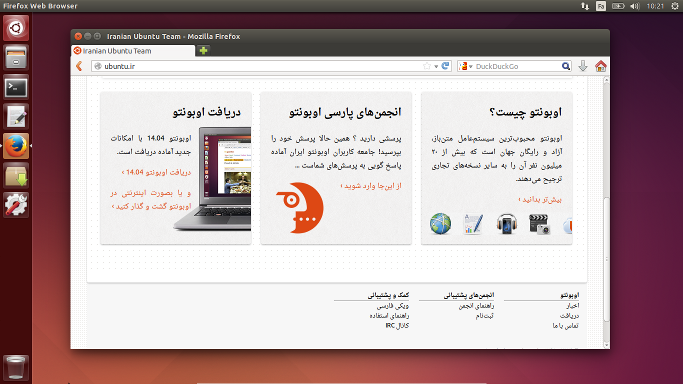
\includegraphics[scale=0.5]{pics/ubuntu-14.04-firefox.png}
\caption{اوبونتو ۱۴٫۰۴ در حال اجرای فایرفاکس}
\label{fig:ubuntu-14.04-firefox}
\end{figure}

\section{مطالعه‌ی بیشتر}
\pagenumbering{arabic}
%\chapter{دانلود اوبونتو}
اوبونتو سیستم‌عاملی آزاد و رایگان می‌باشد که می‌توان آن را از وب‌گاه رسمی آن به نشانی زیر دانلود نمود.

\begin{url-address}
\input{urls/ubuntu_download}
\end{url-address}
 این صفحه از وب‌گاه به صورت زیر است.
\begin{figure}[hbtp]
\centering
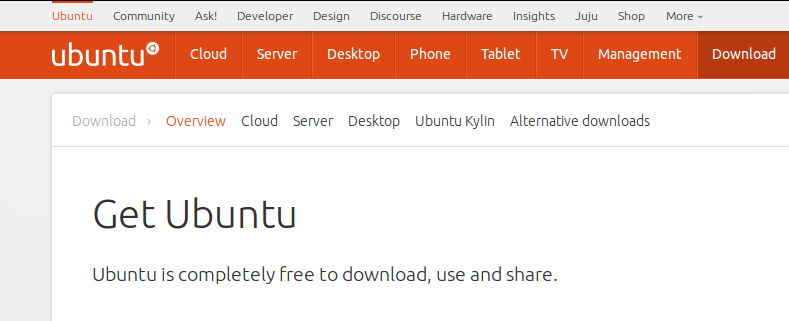
\includegraphics[scale=0.5]{pics/ubuntu-download.png}
\caption{صفحه‌ی دانلود اوبونتو}
\label{fig:ubuntu-download}
\end{figure}

همان‌طور که در عکس قابل مشاهده است، چهار گزینه برای دانلود در دسترس می‌باشد:
\begin{description}
\item[\lr{Ubuntu Desktop}] این ویرایش مخصوص کاربران خانگی و برای استفاده‌ی روزمره است.
\item[\lr{Ubuntu Server}] این ویرایش مخصوص کاربرانی است که قصد ایجاد سرور بر پایه‌ی اوبونتو دارند.
\item[\lr{Ubuntu Cloud}] این ویرایش مخصوص کسانی است که می‌خواهند از اوبونتو برای محیط ابری استفاده کنند.
\item[\lr{Ubuntu Kylin}] این نسخه مخصوص کاربران چینی اوبونتو است
\end{description}
%\input{ch02}
%\chapter{اولین قدم‌ها با اوبونتو}
در این فصل ما به بررسی کارهای ابتدایی با اوبونتو می‌پردازیم.
\section{آشنایی با اجزای مختلف محیط کاربری}
هنگامی که ما برای اولین بار وارد محیط اوبونتو می‌شویم، محیط رومیزی مانند شکل زیر است.

\begin{figure}[hbtp]
\centering
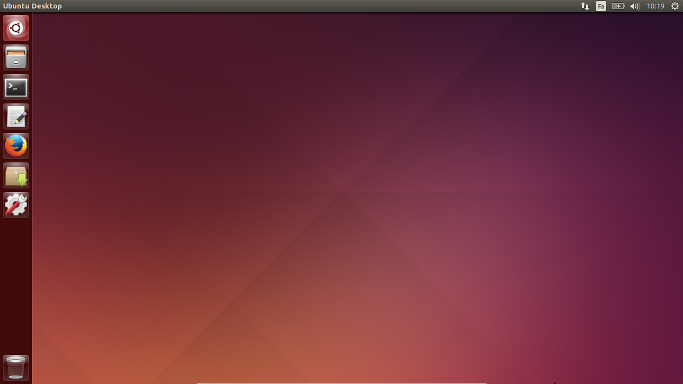
\includegraphics[scale=0.7]{pics/ubuntu-14.04.png}
\caption{محیط رومیزی اوبونتو}
\end{figure}
\subsection{محیط رومیزی}
محیط رومیزی
\footnote{\lr{Desktop Environment}}
پیش‌فرض هنگام نصب اوبونتو، یونیتی
\footnote{\lr{Unity}} 
است. این محیط رومیزی بر پایه‌ی گنوم ۳ کار می‌کند.
\subsection{فایرفاکس}
این مرورگر به صورت پیش‌فرض بر روی اوبونتو نصب می‌باشد.
\subsection{ترمینال}
\subsection{لیبره‌آفیس}
\subsubsection{لیبره‌آفیس رایتر}
\subsubsection{لیبره‌آفیس کلک}
\subsubsection{لیبره‌آفیس ایمپرس}
\section{بروزرسانی}
اولین کاری که می‌توان برای بهبود کارایی سیستم‌عامل انجام داد، به‌روزرسانی سیستم‌عامل است. این امر از طریق‌های متفاوتی قابل انجام است که در این قسمت با استفاده از ترمینال گفته می‌شود.

\begin{latin}
\begin{lstlisting}
$ sudo apt-get update
\end{lstlisting}
\end{latin}

\begin{latin}
\begin{lstlisting}
$ sudo apt-get dist-upgrade
\end{lstlisting}
\end{latin}
\section{نصب نرم‌افزار}
نصب نرم‌افزار در سیستم‌عامل اوبونتو از چند طریق ممکن است. 

\begin{itemize}
\item از طریق نرم‌افزار 
«\lr{Ubuntu Software Center}»
\item از طریق ترمینال و یا
\item از طریق نرم‌افزار \lr{Synaptic Package Manager}.
\end{itemize}

\section{سفارشی سازی محیط رومیزی}
برای سفارشی سازی
\footnote{\lr{customizing}}
محیط رومیزی می‌توان از نرم‌افزار gnome-tweak-tool یا unity-tweak-tool اقدام نمود.

\section{پرسشگان}
\section{مطالعه‌ی بیشتر}

%\input{ch04}
\addcontentsline{toc}{chapter}{واژه‌نامه  انگلیسی به  فارسی}
\chapter*{واژه‌نامه  انگلیسی به  فارسی}
\markboth{واژه‌نامه  انگلیسی به  فارسی}{واژه‌نامه  انگلیسی به  فارسی}

\persiangloss{بنیاد نرم‌افزار آزاد}{Free Software Foundation}
\persiangloss{سیستم کنترل نسخه}{revision control system}
\persiangloss{کد منبع}{source code}
\addcontentsline{toc}{chapter}{واژه‌نامه فارسی به انگلیسی}
\chapter*{واژه‌نامه فارسی به انگلیسی}
\markboth{واژه‌نامه فارسی به انگلیسی}{واژه‌نامه فارسی به انگلیسی}

\englishgloss{revision control system}{سیستم کنترل نسخه}
\englishgloss{source code}{کد منبع}
\end{document}